\section{Conclusiones}

\begin{frame}{Sobre Shadertoy}
\begin{itemize}
    \item Éste fue un taller básico, hay muchas cosas por experimentar y aprender.
    \item Yo empece leyendo \href{https://inspirnathan.com/posts/47-shadertoy-tutorial-part-1}{éste tutorial} y me sirvió mucho. De hecho, éste taller esta basado en el tutorial.
    \item Aunque vimos como usar Ray Marching en el contexto de Shadertoy, ambas cosas no están necesariamente unidas.
    \begin{itemize}
        \item Se pueden hacer escenas en 3D en Shadertoy usando otras técnicas además de Ray Marching.
        \item Se puede utilizar Ray Marching, sin usar el paradigma de \say{Dibujar el mundo en dos triángulos}.
    \end{itemize}
    \item El sitio web de Shadertoy, no es el único entorno donde puedes experimentar con shaders de juguete.
\end{itemize}
\end{frame}

\begin{frame}{Shaders de juguete}
 \begin{itemize}
    \item Puedes extender la plantilla 3D agregando:
    \begin{itemize}
       \item Soft shadows.
       \item Ambient oclusion.
       \item PBR shading.
    \end{itemize}
    \item También puedes investigar acerca de herramientas de Shadertoy no vistas aquí:
    \begin{itemize}
        \item Canales, Buffers, Sonidos y música.
        \item Otras formas de interacción.
    \end{itemize}
    \item Por supuesto, leer shaders escritos por otras personas en Shadertoy.
    \item Hay (al menos) tres \say{familias} de shaders de juguete.
    \begin{enumerate}
       \item Técnicas generativas.
       \item Técnicas de 2D.
       \item Trazadores de rayos.
    \end{enumerate}
  \end{itemize}
\end{frame}


\begin{frame}{Técnicas de 2D dimensiones}
\begin{columns}
\column[t]{0.5\textwidth}
    \begin{itemize}
         \item Puedes leer el \href{https://thebookofshaders.com/05/}{libro de los shaders}: el capítulo de Algorithmic drawing.
         \item Leer el libro de \href{https://natureofcode.com/}{Nature of code}, los primeros capítulos.
         \item Estos recursos cubren \emph{técnicas generales de GC}, que puedes adaptar para hacer shaders de juguete.
     \end{itemize}
\column[t]{0.5\textwidth}
\begin{figure}[htp]
 \centering
 \begin{subfigure}[b]{0.42\textwidth}
   
\includegraphics[width=\textwidth]{img/2D/stainedGlassWindows2}
   \caption{\href{https://www.shadertoy.com/view/3cXSz4}{stained glass windows2}}
 \end{subfigure}
~
 \begin{subfigure}[b]{0.42\textwidth}
   \includegraphics[width=\textwidth]{img/2D/ShaderArtCodingIntroduction}
   \caption{\href{https://www.shadertoy.com/view/mtyGWy}{Coding Introduction}}
 \end{subfigure}
\\
 \begin{subfigure}[b]{0.42\textwidth}
   
\includegraphics[width=\textwidth]{img/2D/VoronoiDistances}
   \caption{\href{https://www.shadertoy.com/view/ldl3W8}{Voronoi - distances}}
 \end{subfigure}
~
 \begin{subfigure}[b]{0.42\textwidth}
   
\includegraphics[width=\textwidth]{img/2D/PrettyHip}
   \caption{\href{https://www.shadertoy.com/view/XsBfRW}{Pretty Hip}}
 \end{subfigure}
 \caption{Propiedad de los respectivos autores}
\end{figure}
\end{columns}
\end{frame}

\begin{frame}{Técnicas generativas}
\begin{columns}
\column[t]{0.5\textwidth}
    \begin{itemize}
         \item El \href{https://thebookofshaders.com/10/}{libro de shaders} el capítulo de funciones generativas.
         \item El libro de \href{https://natureofcode.com/}{Nature of code}, del capítulo 4 en adelante.
         \item Estas también son \emph{técnicas generales de GC}, que puedes adaptar para hacer shaders de juguete.
     \end{itemize}
\column[t]{0.5\textwidth}
\begin{figure}[htp]
 \centering
 \begin{subfigure}[b]{0.42\textwidth}
   
\includegraphics[width=\textwidth]{img/Generative/Grok111}
   \caption{\href{https://www.shadertoy.com/view/wc23Wc}{Grok [111]}}
 \end{subfigure}
~
 \begin{subfigure}[b]{0.42\textwidth}
   \includegraphics[width=\textwidth]{img/Generative/PhantomStarForCineShader}
   \caption{\href{https://www.shadertoy.com/view/ttKGDt}{Phantom Star}}
 \end{subfigure}
\\
 \begin{subfigure}[b]{0.42\textwidth}
   \includegraphics[width=\textwidth]{img/Generative/Seascape}
   \caption{\href{https://www.shadertoy.com/view/Ms2SD1}{Seascape}}
 \end{subfigure}
~
 \begin{subfigure}[b]{0.42\textwidth}
   \includegraphics[width=\textwidth]{img/Generative/Clouds}
   \caption{\href{https://www.shadertoy.com/view/XslGRr}{Clouds}}
 \end{subfigure}
 \caption{Propiedad de los respectivos autores}
\end{figure}
\end{columns}
\end{frame}

\begin{frame}{Shaders que usan técnicas en 3D}
\begin{columns}
\column[t]{0.5\textwidth}
    \begin{itemize}
         \item Leer los tres libros de la colección: \href{https://raytracing.github.io/}{Ray Tracing in One Weekend}.
         \item Ver los videos del canal de \href{https://www.youtube.com/c/InigoQuilez}{Iñigo Quilez en youtube} y leer su \href{https://iquilezles.org/}{sitio web}.
         \item Algún libro de Graficación por computadora.
     \end{itemize}
\column[t]{0.5\textwidth}
\begin{figure}[htp]
 \centering
 \begin{subfigure}[b]{0.42\textwidth}
   \includegraphics[width=\textwidth]{img/3D/Insect}
   \caption{\href{https://www.shadertoy.com/view/Mss3zM}{Insect}}
 \end{subfigure}
~
 \begin{subfigure}[b]{0.42\textwidth}
   \includegraphics[width=\textwidth]{img/3D/OrbitalMegastructure}
   \caption{\href{https://www.shadertoy.com/view/WlKXzm}{Orbital Megastructure}}
 \end{subfigure}
\\
 \begin{subfigure}[b]{0.42\textwidth}
   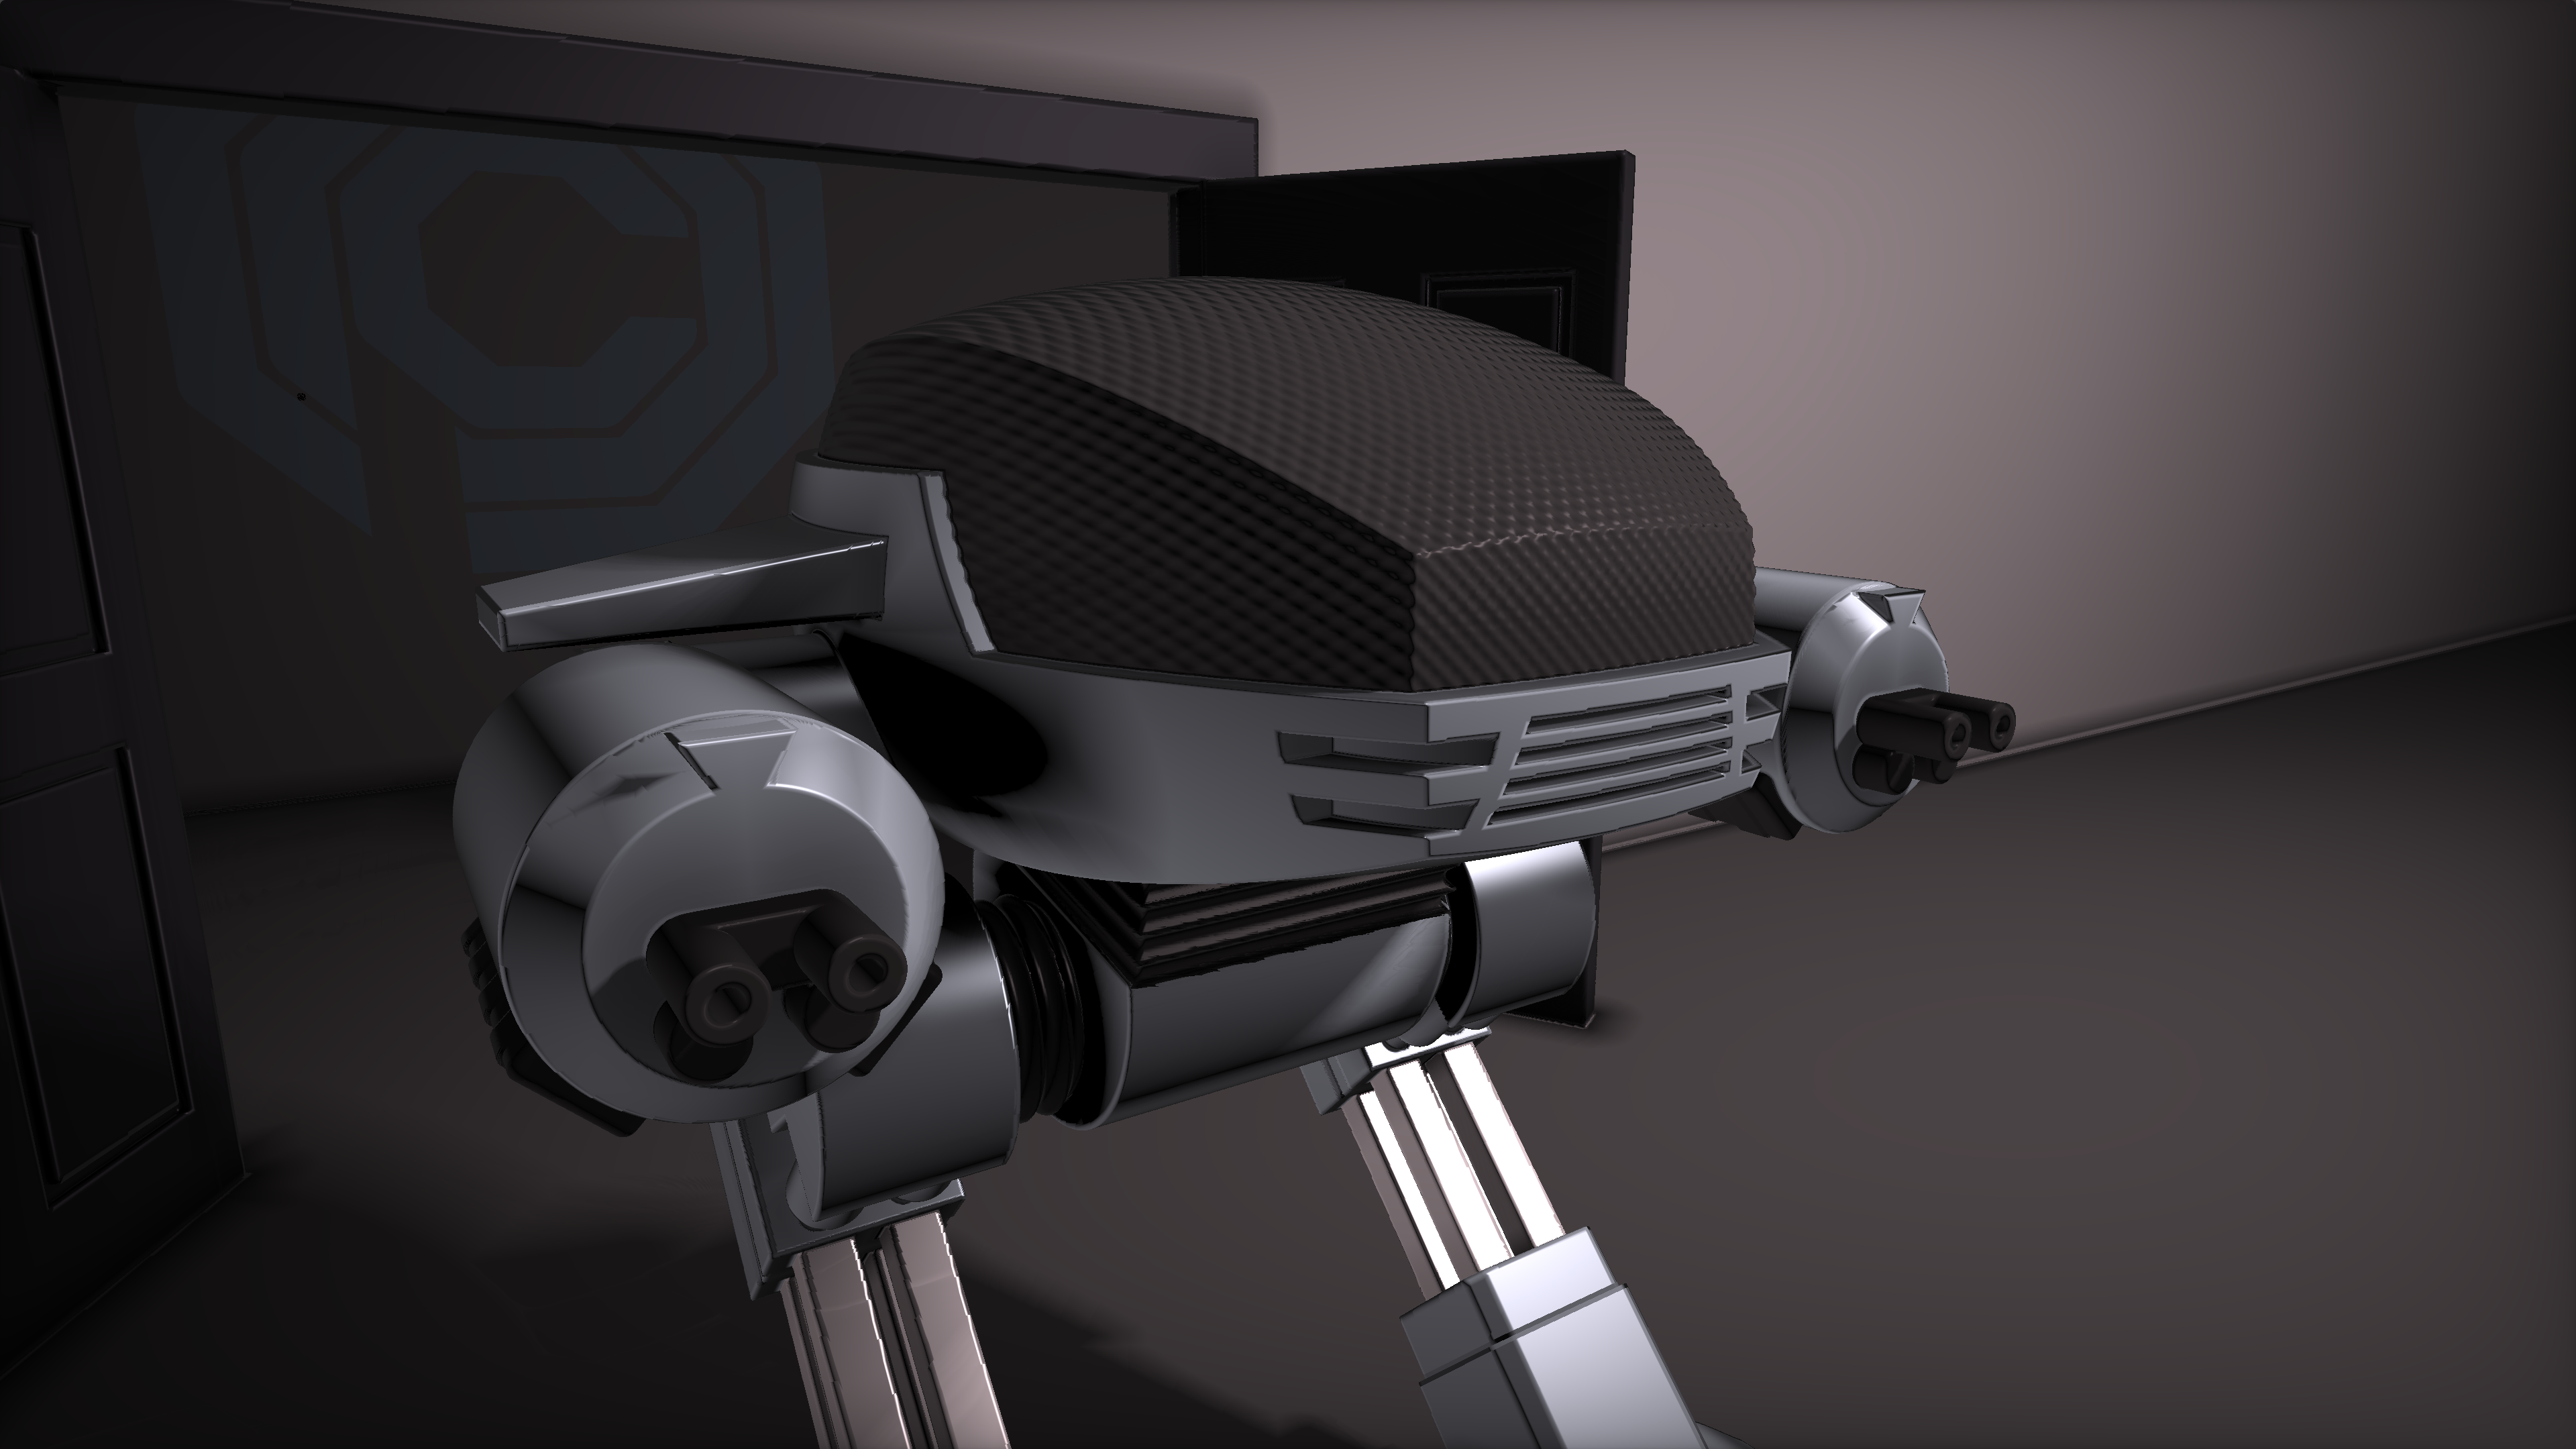
\includegraphics[width=\textwidth]{img/3D/ED-209}
   \caption{\href{https://www.shadertoy.com/view/wsGczG}{ED-209}}
 \end{subfigure}
~
 \begin{subfigure}[b]{0.42\textwidth}
   \includegraphics[width=\textwidth]{img/3D/SpaceAtHome}
   \caption{\href{https://www.shadertoy.com/view/MXS3zy}{Space At Home}}
 \end{subfigure}
 \caption{Propiedad de los respectivos autores}
\end{figure}
\end{columns}
\end{frame}

\begin{frame}{Graficación por computadora en la UNAM}
\begin{columns}
\column[t]{0.5\textwidth}
\begin{itemize}
    \item \href{https://www.fciencias.unam.mx/estudiar-en-ciencias/estudios/licenciaturas/ccomputacion}{Ciencias de la Computación.}
    \begin{itemize}
        \item \href{https://www.fciencias.unam.mx/estudiar-en-ciencias/estudios/licenciaturas/asignaturas/1556/659}{Animación por Computadora}.
        \item \href{https://www.fciencias.unam.mx/estudiar-en-ciencias/estudios/licenciaturas/asignaturas/1556/803}{Graficación por Computadora}.
        \item \href{https://www.fciencias.unam.mx/estudiar-en-ciencias/estudios/licenciaturas/asignaturas/1556/666}{Diseño y Programación de Videojuegos}.
        \item \href{https://www.fciencias.unam.mx/estudiar-en-ciencias/estudios/licenciaturas/asignaturas/1556/771}{Realidad Virtual}.
        \item \href{https://www.fciencias.unam.mx/estudiar-en-ciencias/estudios/licenciaturas/asignaturas/1556/809}{Visualización}.
    \end{itemize}
    \item \href{https://www.cuautitlan.unam.mx/licenciaturas/informatica/}{Informática}
    \begin{itemize}
        \item \href{https://www.cuautitlan.unam.mx/licenciaturas/informatica/}{Seminario de Graficación por Computadora I}.
        \item \href{https://www.cuautitlan.unam.mx/licenciaturas/informatica/descargas/optativas_eleccion/sgcll.pdf}{Seminario de Graficación por Computadora II}.
    \end{itemize}
    \item \href{https://mac.acatlan.unam.mx/}{Matemáticas Aplicadas y Computación}.
    \begin{itemize}
        \item \href{https://mac.acatlan.unam.mx/media/temarios/1644/1055.pdf}{Graficación por Computadora}.
    \end{itemize}
\end{itemize}
\column[t]{0.5\textwidth}
\begin{itemize}
    \item \href{https://www.ingenieria.unam.mx/programas_academicos/licenciatura/computacion.php}{Ingeniería en Computación}.
    \begin{itemize}
        \item Computación Gráfica e Interacción Humano Computadora.
        \item Computación Gráfica Avanzada.
    \end{itemize}
    \item \href{https://www.enesmorelia.unam.mx/licenciaturas/tecnologias-para-la-informacion-en-ciencias/}{Tecnologías para la Información en Ciencias}.
    \begin{itemize}
        \item \href{https://www.enesmorelia.unam.mx/wp-content/uploads/2021/07/Visualizacio\%CC\%81n-3D-de-Informacio\%CC\%81n-Geoespacial.pdf}{Visualización 3D de Información Geoespacial}.
    \end{itemize}
    \item \href{https://www.acatlan.unam.mx/index.php?id=23}{Diseño Gráfico}.
    \begin{itemize}
        \item \href{https://www.acatlan.unam.mx/files/PlanesDeEstudio/DisenoGrafico/7/Optativas/Modelado_y_Animacion_3D.pdf}{Modelado y animación 3D}.
    \end{itemize}
    \item \href{https://fad.unam.mx/oferta-academica/licenciaturas/dcv/}{Diseño y Comunicación Visual}.
    \begin{itemize}
        \item Arte y Producción para Videojuegos.
    \end{itemize}
\end{itemize}
\end{columns}
\end{frame}

\begin{frame}{Graficación por computadora en general}
\begin{itemize}
    \item Leer \href{https://www.amazon.com/Mathematics-Programming-Computer-Graphics-Third/dp/1435458869}{Mathematics for 3D Game Programming and Computer Graphics} y \href{https://link.springer.com/book/10.1007/978-1-84628-997-2}{Geometric Algebra for Computer Graphics}.
    \item Aprender a usar algún framework gráfico. Recomiendo: \href{https://github.com/google/bigwheels}{BigWheels} o \href{https://github.com/google/filament}{Filament}.
    \item Aprender un lenguaje de shaders \href{https://www.amazon.com/OpenGL-Shading-Language-Cookbook-high-quality/dp/1789342252/}{como GLSL} a mas profundidad.
    \item Si buscan inspiración a mi me gusta ver el video de \href{https://www.youtube.com/watch?v=BFld4EBO2RE}{Painting a Landscape with Mathematics}.
\end{itemize}
\begin{figure}[htp]
 \centering
 \begin{subfigure}[b]{0.3\textwidth}
   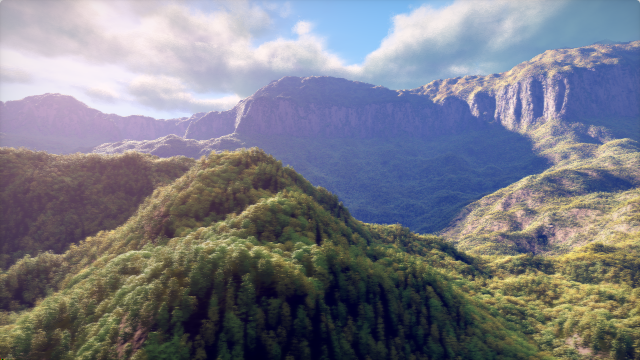
\includegraphics[width=\textwidth]{img/RainForest}
 \end{subfigure}
~
 \begin{subfigure}[b]{0.12\textwidth}
   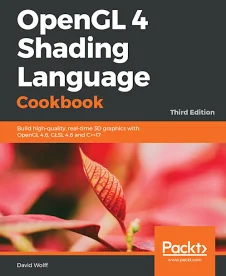
\includegraphics[width=\textwidth]{img/shaderBook}
 \end{subfigure}
\end{figure}
\end{frame}
